% Clast de documento
\documentclass[12pt, letterpaper]{article}

% Paquetes
\usepackage[utf8]{inputenc}
\usepackage[spanish]{babel}
\usepackage{biblatex}
\usepackage{csquotes}
\usepackage{graphicx}
\usepackage{datetime}
\usepackage{lipsum}
\usepackage{hyperref}
\usepackage{fancyhdr}
\usepackage{parskip}
\usepackage{amsmath}
\usepackage{listings}
\usepackage[table,xcdraw]{xcolor}
\usepackage{booktabs}

%------------ 
% Decoración
%------------

% Configuración de colores de python
\lstset{
    language=Python,
    basicstyle=\ttfamily\small,
    keywordstyle=\color{blue},
    commentstyle=\color{green},
    stringstyle=\color{red},
    showstringspaces=false,
    numbers=left,
    numberstyle=\tiny\color{gray},
    frame=single,
    breaklines=true
}

\lstset{
    literate={á}{{\'a}}1 {é}{{\'e}}1 {í}{{\'\i}}1 {ó}{{\'o}}1 {ú}{{\'u}}1
             {Á}{{\'A}}1 {É}{{\'E}}1 {Í}{{\'I}}1 {Ó}{{\'O}}1 {Ú}{{\'U}}1
             {ñ}{{\~n}}1 {Ñ}{{\~N}}1
             {¡}{{!`}}1 {¿}{{?`}}1 % Añade caracteres especiales en español
}

% Configuración de header y footer
\fancyhf{}
\setlength{\headheight}{15.71667pt}
\addtolength{\topmargin}{-3.71667pt}
\fancyhf{}

% Header
\fancyhead[L]{\textsc{\doctitle}}
\renewcommand{\sectionmark}[1]{\markright{#1}}
\fancyhead[R]{\textit{\nouppercase{\rightmark}}}

% Footer
\renewcommand{\footrulewidth}{0.4pt}
\fancyfoot[C]{Página \thepage}

% Título
\newcommand{\doctitle}{Modulación de señales}
\title{\doctitle}
\author{Juan Luis Serradilla Tormos}
\date{\monthname[\month] de \the\year}

% Bibliografía
\addbibresource{test.bib}

% Eliminar sangría
\setlength{\parindent}{0pt}

% Aumentar la separación entre párrafos
\setlength{\parskip}{1em plus 0.5em minus 0.2em}


%-----------
% Documento
%-----------
\begin{document}

% Mostrar header y footer
\pagestyle{fancy}

% Mostrar el título
\maketitle

% Índice
\newpage
\tableofcontents

% Contenido
\newpage
\section{Introducción}
El Internet de las Cosas (IoT) consiste en una red de objetos físicos equipados con hardware y software que les permita conectarse e intercambiar datos a través de una red común. Al ser por tanto la comunicación entre dispositivos imprescindible en el IoT, las tecnologías de comunicación son un tema fundamental en este campo.

Este trabajo explorará las tecnologías de comunicación de los dispositivos IoT centrándose en la modulación de señales. Estas técnicas se utilizan para modificar las señales electromagnéticas para que puedan transmitir información. Por lo tanto, se investigarán sus fundamentos y funcionamiento, las tenoclogías y técnicas actuales, su implementación y los desafíos futuros.


\vspace{1em}
\section{Fundamentos de la Modulación de Señales}

La modulación de señales es un proceso fundamental en los sistemas de comunicación, ya que como se ha mencionado anteriormente la transmisión eficiente y onfiable de los datos es especialmente importante.

En esencia, la modulación de señales consiste en modificar las propiedades de una onda portadora para transmitir información. 

\newpage
\begin{figure}[h]
    \centering
    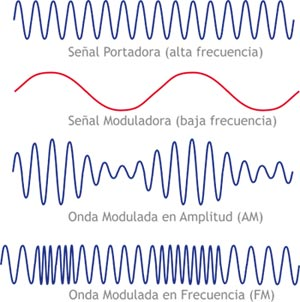
\includegraphics[width=6cm]{images/modulacion_ejemplo.jpg}
    \caption{Ejemplo de modulación de una onda portadora con una onda moduladora de baja frecuencia para transmitir información.}
    \label{fig:modulacion_ejemplo}
\end{figure}

Como se puede ver en la figura \ref{fig:modulacion_ejemplo}, la modulación consta de una onda portadora y una onda moduladora, donde esta onda moduladora portará los datos digitales de los dispoisitvos IoT. Vamos a analizar más en detalle estos dos roles.

\subsection{Frecuencia portadora}
Una señal portadora es una onda eléctrica que puede ser modificada en alguno de sus parámetros por la señal de información para obtener una señal modulada y que se transporta por el canal de comunicaciones. 

Esta onda portadora también ayuda a solucionar el problema del tamaño de las antenas. El tamaño de una antena ($L$) debe ser proporcional a la longitud de la onda ($\lambda$), para así poder apreciar los cambios de la señal. Por ello, tenemos lo siguiente:
\begin{align}
    L \propto \lambda \propto \frac{1}{\nu}
\end{align}
donde $\nu$ es la frecuencia de la señal portadora. Esta característica hace que se puedan utilizar antenas de tamaño práctico para la transmisión inalámbrica.

Esta onda portadora también ayuda a que la señal enviada sea resistente al ruido.

\subsection{Frecuencia moduladora}
La onda moduladora es la onda que contiene la información digital que se quiere transmitir. Esta suele ser de una frecuencia más baja, por lo que necesita a la onda portadora para poder ser transmitida. El objetivo de esta onda es modificar algún parámetro de la onda portadora, como la amplitud, la frecuencia o la fase, para que la información pueda ser transmitida a través del canal de comunicación.

Las dos formas básicas de modulación son:
\begin{itemize}
    \item \textbf{Modulación de amplitud:} Este tipo de modulación consiste en variar el valor de la amplitud de la onda portadora en función de la onda moduladora. 

    \item \textbf{Modulación angular:} Este tipo de modulación consiste en variar el ángulo de la onda portadora. Para ello, se puede modificar tanto la frecuencia como la fase, pero manteniendo siempre la amplitud constante.
\end{itemize}

Otra forma de clasificar a la modulación es en función de cómo se realiza este proceso: de forma digital o de forma analógica. 

\begin{itemize}
    \item \textbf{Modulación analógica:} Este tipo de modulación realiza cambios continuos en la señal portadora, variando los parámetros de amplitud, frecuencia o fase de forma proporcional a la señal original. Podemos distinguir:
    \begin{itemize}
        \item Modulación AM
        \item Modulación FM
        \item Modulación PM
    \end{itemize}

    \item \textbf{Modulación digital:} En este tipo de modulación la señal moduladora es discreta (0 o 1). La información se codifica en símbolos (grupos de bits) que modifican la señal portadora de forma discontinua. Podemos distinguir:
    \begin{itemize}
        \item Modulación ASK
        \item Modulación FSK
        \item Modulación PSK
        \item Modulación QAM
    \end{itemize}
\end{itemize}

\subsection{Modulación digital sobre analógica}
A pesar de que existan dos tipos de modulación, en el contexto del IoT la modulación digital es la más utilizada. Esto se debe a varias razones:
\begin{itemize}
    \item \textbf{Sensibilidad al ruido:} La modulación analógica, especialmente AM, es más susceptible al ruido y las interferencias, lo que puede degradar la calidad de la señal transmitida. En entornos IoT donde los dispositivos pueden operar en condiciones ruidosas o con señales débiles, la robustez de la modulación digital ofrece una ventaja significativa.
    \item \textbf{Menor eficiencia espectral:} En general, las técnicas de modulación digital pueden ofrecer una mayor eficiencia espectral en comparación con las analógicas, lo que permite transmitir más datos dentro de un ancho de banda limitado. Esto es crucial en el espectro de radiofrecuencia cada vez más congestionado donde operan muchos dispositivos IoT.
    \item \textbf{Integración con sistemas digitales:} Dado que los dispositivos IoT operan con datos digitales, la modulación digital permite una integración más sencilla y directa con los circuitos y procesadores digitales. La conversión de señales analógicas a digitales y viceversa añade complejidad y puede introducir pérdidas.
    \item \textbf{Seguridad y cifrado:} Las técnicas de modulación digital se prestan mejor a la implementación de mecanismos de seguridad como el cifrado, que es cada vez más importante para proteger la confidencialidad e integridad de los datos transmitidos por los dispositivos IoT.
    \item \textbf{Eficiencia energética:} Muchas técnicas de modulación digital están diseñadas para ser energéticamente eficientes, lo cual es un requisito fundamental para los dispositivos IoT que funcionan con baterías y necesitan operar durante períodos prolongados.
\end{itemize}

\vspace{1em}
\section{Técnicas de modulación digital}
A continuación, se van a analizar las diferentes técnicas de modulación digital que se usan en el IoT.

\subsection{Modulación ASK y OOK}
La modulación ASK es un tipo de modulación de amplitud, por lo que los datos se representan variando la amplitud de la onda portadora. OOK por su parte es una forma de ASK donde la señal portadora se apaga y enciende para representar los bits 0 y 1. 

En ASK, la presencia de una onda portadora a una amplitud específica representa un bit 1, mientras que una amplitud diferente o la ausencia de la onda representa un bit 0. La fórmula para representar esta onda es la siguiente:
\begin{align}
    U_{ASK}(t) = A \Big[1 \pm \frac{V(t)}{A} \Big] \cos(2\pi \nu_p t) = 
    A [1 \pm m(t)] \cos(2\pi \nu_p t) \label{eq:ask}
\end{align}

donde $V(t)$ es la señal moduladora, $A$ es la amplitud de la portadora, $\nu_p$ es la frecuencia de la portadora y $m(t)$ es la señal moduladora normalizada.

Se puede ver en la ecuación~\ref{eq:ask} que la amplitud de la señal portadora se modula en función de la seál portadora $V(t)$, pudiendo aumentar o disminuir dependiendo de cómo se haga la modulación.

\begin{figure}[h]
    \centering
    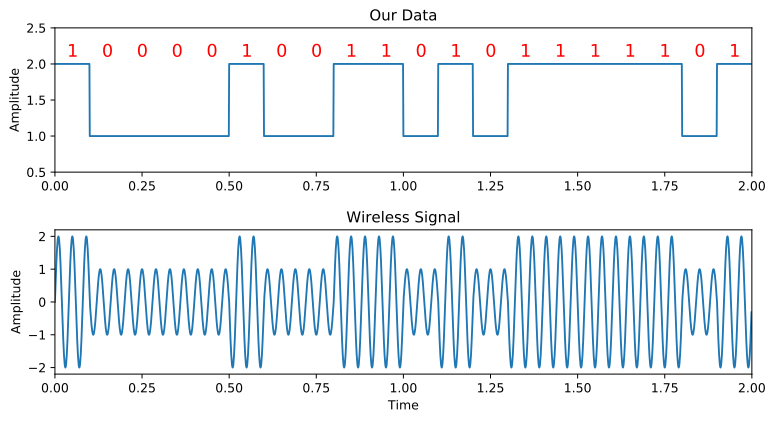
\includegraphics[width=9cm]{images/ASK.png}
    \caption{Ejemplo de modulación ASK.}
    \label{fig:ask}
\end{figure}

\newpage
Este tipo de modulación tiene sus ventajas y desventajas.
\begin{itemize}
    \item \textbf{Ventajas:}
    \begin{itemize}
        \item Es un método simple y fácil de implementar. Esto se debe a que, al solo tener que variar la amplitud moduladora para representar bits, solo hacen falta componentes simples como osciladores e interruptores. 
        \item Este método, en especial OOK, es muy eficiente  energéticamente. Esto se debe a que solo se transmite información cuando hay un "1", a diferencia de otros métodos que requieren la energía constante para mantener activa la portadora.
    \end{itemize}

    \item \textbf{Desventajas:}
    \begin{itemize}
        \item Es susceptible a las variaciones de amplitud y al ruido, debido a que es una transformación lineal. Es decir, si la amplitud de la señal portadora se ve afectada por el ruido, la señal modulada también se verá afectada de igual forma. Debido a esta distorsión los rangos de amplitud son limitados.
        \item Tiene menor eficiencia espectral que otros tipos de modulación. Esto se debe a varias razones; una de ellas es que transmite solo 1 bit por símbolo, en comparación con otros métodos como QAM que transmite 4 bits por símbolo. Esto a su vez hace que se necesiten más símbolos para enviar la misma cantidad de información, lo que amplia el ancho de banda necesario.
    \end{itemize}
\end{itemize}

\newpage
\section{Tecnologías de Comunicación}

\newpage
\section{Técnicas de modulación}

\newpage
\section{Implementación y aplicación en IoT}

\newpage
\section{Desafíos y perspectivas futuras}

\newpage
\section{Conclusiones}

\end{document}
